% !TEX program = pdflatex
\documentclass[12pt]{article}

\IfFileExists{spanish.ldf}{
    \usepackage[spanish,es-nodecimaldot]{babel}
}{
    \usepackage{babel}
    \renewcommand{\figurename}{Figura}
    \renewcommand{\tablename}{Tabla}
}

\usepackage[utf8]{inputenc}
\usepackage[T1]{fontenc}
\IfFileExists{newtxtext.sty}{\usepackage{newtxtext,newtxmath}}{}
\usepackage[a4paper,margin=2.5cm]{geometry}
\IfFileExists{setspace.sty}{\usepackage{setspace}}{}
\usepackage{graphicx}
\usepackage{amsmath}
\usepackage{float}
\usepackage[hidelinks]{hyperref}
\urlstyle{same}
\IfFileExists{xurl.sty}{\usepackage{xurl}}{}
\usepackage{array}
\usepackage{longtable}
\usepackage{tabularx}
\usepackage{pdflscape}
\IfFileExists{microtype.sty}{\usepackage{microtype}}{}
\usepackage{tikz}
\usetikzlibrary{positioning,arrows.meta}

\IfFileExists{setspace.sty}{
    \setstretch{1.15}
}{
    \linespread{1.15}
}

\renewcommand{\arraystretch}{1.15}
\graphicspath{{./}{imagenes_informe/}}
\setlength{\emergencystretch}{3em}
\setlength{\parindent}{0pt}
\setlength{\parskip}{0.7em}
\renewcommand{\contentsname}{Índice}
\renewcommand{\refname}{Referencias}
\setcounter{secnumdepth}{1}

\newcommand{\imagenreporte}[3]{%
    \begin{figure}[H]
    \centering
    \includegraphics[width=#2\textwidth]{#1}
    \caption{#3}
    \end{figure}
}

\begin{document}

\hypersetup{pageanchor=false}
\begin{titlepage}
\thispagestyle{empty}
\vspace*{1.2cm}

\begin{center}
{\Large \textbf{UNIVERSIDAD DEL VALLE DE GUATEMALA}}\\[0.4cm]
{\normalsize Facultad de Ingeniería}\\
{\normalsize Modelación y Simulación}\\
{\normalsize Semestre II -- 2026}\\[1.2cm]

% \IfFileExists no usa \graphicspath: se busca el logo junto al .tex y en imagenes_informe/.
\IfFileExists{logo.png}{
    
\includegraphics[width=0.42\textwidth]{logo.png}\par
    \vspace{1.4cm}
}{\IfFileExists{imagenes_informe/logo.png}{
    
\includegraphics[width=0.42\textwidth]{imagenes_informe/logo.png}\par
    \vspace{1.4cm}
}{
    \vspace*{4.4cm}
}}

{\LARGE \textbf{Proyecto 2}}\\[0.4cm]
{\Large \textbf{Simulación y optimización del riego en macetas}}\\[0.3cm]
{\large Balance de agua, enjambre de partículas y evaluación de políticas}
\end{center}

\vfill

\begin{flushright}
\textbf{Integrantes:}\\
Nájera Marakovits, Ingrid Nina Alessandra -- 231088\\
Ramírez Velásquez, Diego Alejandro -- 23601\\
Canastuj Matías, Eliazar José Pablo -- 23384\\
Escalante Sánchez, Nelson Estuardo -- 22046
\end{flushright}

\end{titlepage}

\pagenumbering{arabic}
\hypersetup{pageanchor=true}

\section*{Resumen}

Se estudió el uso de agua en macetas mediante un balance de masa y una política de riego por umbrales. El modelo se ajustó con pesajes publicados de Ensete ventricosum. Se implementaron Euler y Runge--Kutta de cuarto orden, y se utilizó un enjambre de partículas para elegir cuándo y cuánto regar. En 30 pares de simulaciones de siete días, la política elegida redujo el agua media en 501.2 mL frente a una dosis fija. El ahorro medio por par fue de 19.4\,\%. La propuesta cumplió las restricciones en 29 de 30 ejecuciones normales y falló en todas al aumentar las pérdidas un 20\,\%. El ahorro depende del arranque y de la forma de representar el drenaje.

\section{Problema y objetivo}

Una dosis fija puede superar el agua que perdió una maceta y generar drenaje. También puede resultar insuficiente si aumentan las pérdidas. El peso permite seguir estos cambios y decidir el riego con una medida del déficit.

La pregunta central es si una política por umbrales puede reducir el agua aplicada frente a un riego fijo, manteniendo el déficit por debajo de un límite común. Se busca minimizar el volumen total por maceta durante siete días, incluida la reposición final al estado inicial. Esta reposición evita atribuir ahorro a terminar con menos agua almacenada.

El sistema comprende la maceta, el agua retenida, las pérdidas y las decisiones de riego. Las entradas son las dosis y las condiciones que modifican las pérdidas. Las salidas son el déficit, el consumo y el drenaje. Se excluyen crecimiento, rendimiento y salud de la planta.

\section{Fuente y preparación de las observaciones}

Se utilizó el conjunto de Chase de 2026, disponible en Zenodo bajo licencia CC BY 4.0 \cite{chase}. Los pesajes de la plataforma Phenospex abarcan del 11 de julio al 6 de agosto de 2024. Se seleccionó el secado del 24 de julio al 6 de agosto y se tomaron las lecturas más cercanas a las 07:00, 13:00 y 19:00.

Las mediciones son de terceros: el sistema real es este ensayo documentado y los pesajes se identifican como datos públicos en todo el repositorio.

De 22 plantas sometidas a estrés hídrico se excluyó una con subidas de masa mayores que 50 g en tres horas, señal de aportes de agua sin registro. Quedaron 21 macetas y 793 lecturas. El control de calidad dejó 61 advertencias por aumentos nocturnos de masa, que se conservaron sin corregir las mediciones. Las primeras 382 lecturas se destinaron al ajuste y las 411 restantes a validación, con ventanas consecutivas de siete días.

\begin{table}[H]
\centering
\caption{Origen de los datos utilizados}
\small
\begin{tabularx}{\textwidth}{|l|X|X|}
\hline
Tipo & Datos & Uso \\
\hline
Público, real & Pesajes cada 15 min de Chase (2026) \cite{chase} & Calibración, validación y referencia de la plataforma \\
\hline
Estimado & Riego de las plantas control, error de lectura y variación diaria, calculados a partir de los pesajes públicos & Referencia de riego, límites y escenarios \\
\hline
Sintético & 30 realizaciones del factor diario y del error de lectura, generadas con semillas registradas & Repeticiones de la evaluación \\
\hline
Documentado & Agua aplicada con riego fijo y por tensiómetro en Lieth \cite{lieth} & Antecedente del control del riego \\
\hline
\end{tabularx}
\end{table}

La referencia de masa es la primera lectura del periodo de estrés. No se midió la capacidad máxima de retención. La hora original se conservó con un desfase nominal de seis horas al oeste de UTC, porque la fuente no declara zona horaria. La variación de masa se atribuye principalmente al agua. El trabajo de Lieth sirve como antecedente del control del riego mediante mediciones \cite{lieth}.

\section{Modelo de balance de agua}

El déficit expresa la diferencia de masa en mL. Se adopta una densidad del agua de 1 g/mL.

\begin{equation*}
D=\frac{M_{\mathrm{ref}}-M}{\rho_w}
\end{equation*}

\begin{table}[H]
\centering
\caption{Variables y parámetros principales}
\begin{tabularx}{\textwidth}{|l|l|X|}
\hline
Símbolo & Unidad & Significado \\
\hline
$D$ & mL & Déficit respecto de la masa de referencia \\
\hline
$M$, $M_{\mathrm{ref}}$ & g & Masa observada y masa de referencia \\
\hline
$a$ & mL/h & Pérdida al inicio del rango de déficit \\
\hline
$b$ & h$^{-1}$ & Cambio de la pérdida con el déficit \\
\hline
$q_t$, $u_t$ & Sin unidad & Factor horario y variación diaria de pérdidas \\
\hline
$I$, $Q$ & mL & Agua aplicada y agua drenada en un evento \\
\hline
\end{tabularx}
\end{table}

Entre riegos, el déficit aumenta según

\begin{equation*}
\frac{dD}{dt}=u_t q_t\max\{0,a+bD\}.
\end{equation*}

El factor horario es uno entre 06:00 y 18:00 y cambia durante la noche. Un valor negativo de $b$ reduce la pérdida al secarse la maceta. El modelo agrupa evaporación y transpiración.

El riego repone el déficit y el exceso se considera drenaje instantáneo.

\begin{equation*}
Q=\max\{0,I-D^{-}\}, \qquad D^{+}=\max\{0,D^{-}-I\}.
\end{equation*}

\begin{figure}[H]
\centering
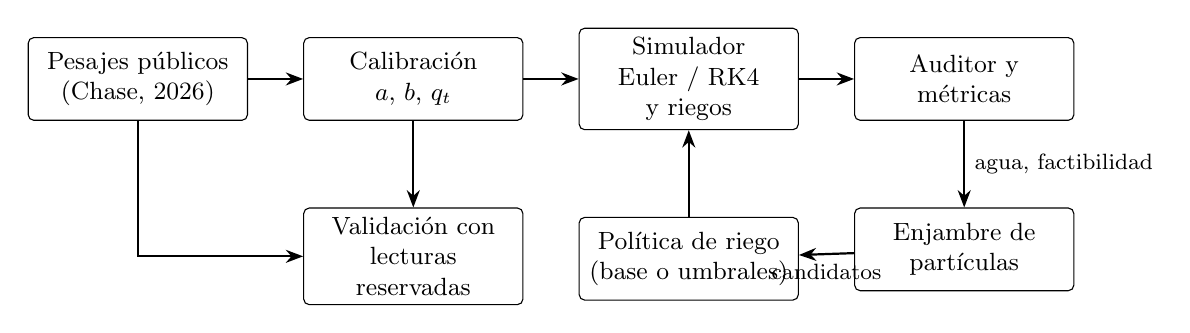
\begin{tikzpicture}[
    node distance=0.55cm and 0.7cm,
    caja/.style={draw, rounded corners=2pt, align=center, minimum height=1.05cm, text width=2.55cm, font=\small},
    flecha/.style={-{Stealth[length=2.2mm]}, thick}]
\node[caja] (datos) {Pesajes públicos\\(Chase, 2026)};
\node[caja, right=of datos] (ajuste) {Calibración\\$a$, $b$, $q_t$};
\node[caja, right=of ajuste] (sim) {Simulador\\Euler / RK4\\y riegos};
\node[caja, right=of sim] (met) {Auditor y\\métricas};
\node[caja, below=1.1cm of sim] (pol) {Política de riego\\(base o umbrales)};
\node[caja, below=1.1cm of met] (pso) {Enjambre de\\partículas};
\node[caja, below=1.1cm of ajuste] (val) {Validación con\\lecturas reservadas};
\draw[flecha] (datos) -- (ajuste);
\draw[flecha] (ajuste) -- (sim);
\draw[flecha] (sim) -- (met);
\draw[flecha] (pol) -- (sim);
\draw[flecha] (met) -- node[right, font=\footnotesize] {agua, factibilidad} (pso);
\draw[flecha] (pso) -- node[below, font=\footnotesize] {candidatos} (pol);
\draw[flecha] (ajuste) -- (val);
\draw[flecha] (datos) |- (val);
\end{tikzpicture}
\caption{Relación entre los componentes del sistema}
\end{figure}

La calibración usa solo la ventana de ajuste. El simulador recibe los parámetros y una política; el auditor comprueba las restricciones sobre la trayectoria. El enjambre propone candidatos, recibe su consumo y factibilidad, y devuelve la política seleccionada.

\section{Calibración y simulación}

Se ajustaron tres formas de pérdida mediante mínimos cuadrados de SciPy. La primera usa una tasa constante, la segunda distingue día y noche y la tercera añade la dependencia del déficit. Se eligió la forma más simple entre las que quedaron a dos unidades del menor AICc. El ajuste utilizó solo intervalos de secado de la primera ventana y 500 remuestreos de días completos para estimar incertidumbre.

Los archivos de calibración seleccionan dependencia del déficit en 17 macetas y tasas por bloques en cuatro. En 15 de las 21 macetas, el intervalo de confianza del 95\,\% de $a$ excluye el valor agrupado, por lo que se usaron parámetros por maceta. Para la optimización se tomó E12, la más cercana a la mediana de los parámetros estandarizados de las 17 macetas con dependencia del déficit. Sus valores son $a=28.23$ mL/h, $b=-0.01022$ h$^{-1}$ y factor nocturno de 0.0253.

Euler actualiza el estado con la pendiente al inicio de cada paso. Runge--Kutta de cuarto orden combina cuatro pendientes y ofrece mayor precisión en tramos suaves \cite{euler,rk4}. Se utilizó un paso máximo de 0.25 h. Los riegos, las revisiones y los cambios horarios se procesaron en sus tiempos exactos, separados de la integración continua.

La verificación incluyó pérdida nula, tasa constante, una solución exponencial y conservación en los riegos. Al reducir el paso a la mitad, el error de Euler mostró orden cercano a uno y el de Runge--Kutta cercano a cuatro. El residuo máximo del balance en las 120 evaluaciones fue de $4.1\times10^{-12}$ mL. Estas pruebas comprueban el cálculo, mientras la validación contrasta las predicciones con los pesajes.

\section{Optimización de la política de riego}

El enjambre de partículas, conocido como PSO, desplaza un grupo de soluciones según su experiencia individual y la mejor solución del grupo \cite{kennedy}. Cada candidato contiene el umbral de activación, el déficit objetivo y la dosis máxima. Los valores se representan en coordenadas entre cero y uno y luego se convierten a múltiplos de 5 mL.

El objetivo es minimizar el promedio de agua aplicada, incluida la reposición final. Se exige un déficit máximo de 520 mL, hasta 750 mL por evento y por día, y no más de tres riegos diarios en las horas de revisión. El límite de déficit procede del máximo de 517 mL observado en las plantas control, redondeado. Es un límite de operación y no una garantía de bienestar vegetal.

La velocidad y la posición de cada partícula se actualizan mediante

\begin{align*}
\mathbf{v}_{k+1}&=w\mathbf{v}_k+c_1\mathbf{r}_1\odot\left[\mathbf{p}_k-\mathbf{x}_k\right]
+c_2\mathbf{r}_2\odot\left[\mathbf{g}_k-\mathbf{x}_k\right],\\
\mathbf{x}_{k+1}&=\mathbf{x}_k+\mathbf{v}_{k+1}.
\end{align*}

Aquí $\mathbf{p}_k$ es la mejor posición individual y $\mathbf{g}_k$ la mejor del grupo. Los vectores $\mathbf{r}_1$ y $\mathbf{r}_2$ contienen sorteos uniformes entre cero y uno. Se compararon inercias de 0.7 y 0.4, con $c_1=c_2=1.4$ y velocidad máxima de 0.2. La documentación de PySwarms y el análisis de Innocente y Sienz orientaron estas decisiones \cite{pyswarms,innocente}.

Cada búsqueda tuvo diez partículas y seis iteraciones, con 60 evaluaciones incluida la población inicial. Se realizaron 30 búsquedas por variante y otras 30 con búsqueda aleatoria bajo el mismo presupuesto. Dos escenarios se usaron para buscar y tres distintos para seleccionar. Un auditor independiente revisó las restricciones antes de comparar el consumo.

PSO permite trabajar sin derivadas y con decisiones que cambian por saltos. Puede estancarse, depende de las semillas y puede ajustarse demasiado a pocos escenarios. La búsqueda aleatoria obtuvo consumos semejantes, de modo que no se demostró una ventaja clara de PSO. El equipo implementó el enjambre, las políticas, los integradores y la auditoría. SciPy se utilizó para el ajuste, NumPy para los cálculos y sorteos, pandas para las tablas y Matplotlib para las figuras.

\section{Diseño experimental y validación}

La base aplica 325 mL diarios a las 07:00. Reproduce el riego diario fijo que la plataforma dio a sus plantas control, y su dosis es la pérdida de 24 h de E12 partiendo de déficit cero (326.4 mL), redondeada a 5 mL. La propuesta seleccionada usa activación de 365 mL, objetivo de 350 mL y dosis máxima de 150 mL. Se mantuvo fija durante la evaluación.

Se compararon B0 y O0 con pérdidas normales, y B1 y O1 con pérdidas aumentadas un 20\,\%. B identifica la base y O la propuesta. Cada condición tuvo 30 repeticiones, con semillas de 13001 a 13030. Ambas políticas recibieron las mismas variaciones por semilla. El factor diario siguió una distribución lognormal de media uno y coeficiente de variación de 0.083. Este valor es la variación entre días de la razón entre pérdida observada y predicha, tomando la mediana entre macetas en los cinco días completos de la ventana de ajuste. El error de lectura siguió una distribución normal de media cero y desviación de 0.397 mL. Se estimó con la dispersión de las diferencias nocturnas de 15 min dividida entre $\sqrt{2}$, porque la fuente no informa una verificación de balanza.

El horizonte fue del 31 de julio al 7 de agosto de 2024, con déficit inicial cero. Al terminar se repuso el agua necesaria para recuperar ese estado. Se registraron consumo, drenaje, déficit máximo, tiempo sobre el límite y cumplimiento de restricciones.

Para validar el secado se inició cada maceta con su primera lectura de la segunda ventana y se predijo el resto sin recalibrar ni reiniciar. Se compararon 390 lecturas. El error absoluto medio fue de 172.36 mL, la raíz del error cuadrático medio de 308.27 mL y el sesgo de +157.30 mL. El error fue mayor donde el secado posterior superó el rango observado durante el ajuste.

\begin{table}[H]
\centering
\caption{Error de validación según la forma de pérdida seleccionada}
\small
\begin{tabularx}{\textwidth}{|X|r|r|r|}
\hline
Forma seleccionada en el ajuste & Macetas & MAE mediano en mL & MAE / déficit medio \\
\hline
Con dependencia del déficit & 17 & 59.7 & 3.7\,\% \\
\hline
Sin dependencia del déficit & 4 & 597.0 & 27.7\,\% \\
\hline
Todas, por observación & 21 & 172.4 & 9.7\,\% \\
\hline
\end{tabularx}
\end{table}

En todas las macetas la ventana de validación alcanzó déficits mayores que los del ajuste. Donde el ajuste identificó la reducción de pérdidas con el secado, el modelo extrapoló con un error mediano de 3.7\,\% del déficit. En las cuatro macetas con pérdida constante sobrestimó el secado posterior. La regla de selección no se modificó después de observar estos errores.

\imagenreporte{04_validation_all.png}{1}{Predicciones y errores de validación en las 21 macetas}

La cercanía a la diagonal indica mejor correspondencia. El error varía entre macetas y hay una tendencia a sobrestimar el déficit. Esta validación evalúa el secado, sin comprobar la respuesta al riego ni el drenaje.

\section{Resultados}

La tabla muestra el consumo medio y su desviación estándar. El déficit máximo corresponde a la media de los máximos de cada ejecución. El agua total incluye la reposición final.

\begin{table}[H]
\centering
\caption{Evaluación por maceta durante siete días}
\small
\begin{tabularx}{\textwidth}{|l|>{\centering\arraybackslash}X|r|r|r|}
\hline
Condición & Agua total en mL & Drenaje en mL & Déficit en mL & Cumplen \\
\hline
B0 & $2586.9\pm30.9$ & 324.2 & 363.8 & 30/30 \\
\hline
O0 & $2085.7\pm54.0$ & 0.0 & 508.0 & 29/30 \\
\hline
B1 & $2845.8\pm42.1$ & 286.0 & 586.6 & 1/30 \\
\hline
O1 & $2478.4\pm62.7$ & 0.0 & 542.2 & 0/30 \\
\hline
\end{tabularx}
\end{table}

\imagenreporte{01_system.png}{0.96}{Trayectoria de la base y la propuesta en una misma semilla}

La propuesta riega con dosis menores y conserva un déficit mayor entre revisiones. El ahorro medio de los 30 pares fue de $501.2\pm38.4$ mL, con una media porcentual de 19.4\,\%. En los 29 pares donde ambas políticas cumplieron, fue de 503.1 mL y 19.5\,\%. La ejecución restante alcanzó 533.24 mL de déficit, por encima del límite de 520 mL.

\imagenreporte{02_policies.png}{0.96}{Agua aplicada con reposición final y variación del drenaje}

De la reducción media, 324.2 mL corresponden a menos drenaje y 177.0 mL a una menor pérdida predicha al mantener la maceta más seca. Esta segunda parte depende del valor negativo de $b$ y no permite concluir que la planta conserve el mismo rendimiento.

\imagenreporte{03_sensitivity.png}{0.96}{Consumo y cumplimiento al aumentar las pérdidas un 20 por ciento}

Con mayores pérdidas, ninguna ejecución de la propuesta cumplió todas las restricciones. La base cumplió en una sola. Aunque O1 pasó menos tiempo sobre el límite que B1, su menor consumo no constituye una mejora aceptable bajo esas condiciones.

\section{Comparación con las plantas control y discusión}

El riego de las dos plantas que permanecieron como control se estimó mediante sus aumentos nocturnos de masa, del 24 de julio al 5 de agosto. El promedio fue de 273.1 mL por maceta al día. Es una cota inferior porque no incluye pérdidas simultáneas ni agua que pudo drenar. La referencia corresponde a otros genotipos, mientras las políticas se simularon con E12.

\begin{table}[H]
\centering
\caption{Referencia de la plataforma y resultados normales de simulación}
\small
\begin{tabularx}{\textwidth}{|X|r|r|r|r|r|}
\hline
Medida & Referencia & Base & Propuesta & Cambio & Cambio en \% \\
\hline
Agua por día en mL & 273.1 & 369.6 & 298.0 & $-71.6$ & $-19.4$ \\
\hline
Déficit máximo en mL & 517.0 & 363.8 & 508.0 & $+144.1$ & $+39.6$ \\
\hline
\end{tabularx}
\end{table}

El cambio se calcula como propuesta menos base, y el porcentaje respecto de la base. La referencia proviene de las plantas control de la misma plataforma y es una medición estimada, no una simulación. La propuesta redujo el consumo en 71.6 mL diarios frente a la base, un 19.4\,\% menos. La base quedó un 35.3\,\% por encima del riego estimado de control. La comparación tiene diferencias de almacenamiento, ya que las simulaciones incluyen reposición final y la referencia no impone ese cierre. Además, el máximo de control se compara con una media de máximos simulados.

El arranque tuvo un efecto importante. La base recibió el primer riego con un déficit medio de solo 32.55 mL y drenó 292.45 mL. Ese evento reunió el 90.2\,\% de su drenaje total. En una comprobación adicional, omitir únicamente ese primer riego redujo el ahorro frente a la misma propuesta a 181.4 mL, cerca del 8.0\,\%. Esta comprobación se realizó después de la evaluación y muestra sensibilidad al arranque, sin reemplazar el diseño inicial.

Quedan otras fuentes de incertidumbre. La masa inicial del secado no demuestra la capacidad máxima de retención, aunque el modelo la utiliza como límite para drenar. El ruido se estimó con el periodo completo de estrés y la comparación mantuvo fijos los parámetros ajustados. Las 30 semillas describen variación dentro del simulador y no equivalen a 30 plantas adicionales. Las políticas no se aplicaron a las macetas de la plataforma.

\section{Conclusiones}

El balance permitió simular el secado y comparar políticas con unidades, restricciones y condiciones comunes. La verificación numérica fue consistente. La validación con lecturas reservadas mostró buen ajuste donde se identificó la dependencia del déficit y errores importantes en las cuatro macetas con pérdida constante.

\begin{itemize}
\item \textbf{¿Qué mejoró?} El agua total aplicada por maceta, incluida la reposición final. La mejora proviene sobre todo de eliminar el drenaje de la dosis fija.
\item \textbf{¿Cuánto mejoró?} 501.2 mL en siete días (19.4\,\%) en los 30 pares, y 503.1 mL (19.5\,\%) en los 29 pares en que ambas políticas cumplieron. Sin el primer riego de la base, el ahorro baja a cerca del 8\,\%.
\item \textbf{¿Bajo qué condiciones?} Con las pérdidas estimadas para la ventana de ajuste, la maceta E12 y un límite de 520 mL. Con pérdidas 20\,\% mayores ninguna política fue aceptable.
\item \textbf{¿Qué tan confiable es la comparación?} Ambas políticas compartieron escenarios, semillas, restricciones y cierre del balance, y un auditor independiente comprobó las restricciones. La mejora es simulada: no se aplicó a plantas reales y depende de un modelo con error de validación de 3.7\,\% a 27.7\,\% según la maceta.
\item \textbf{¿Qué limitaciones permanecen?} Datos de terceros y de una sola maceta representativa; riego de referencia estimado; drenaje instantáneo; sensibilidad al arranque; parte del ahorro depende de $b<0$; y no se comprobó que un mayor déficit conserve el rendimiento vegetal.
\end{itemize}

Para este sistema se recomienda no adoptar la política tal como quedó. Antes conviene añadir un margen de seguridad al límite de 520 mL, reajustarla si aumenta la demanda y evaluar el arranque con un primer riego proporcional al déficit. Cualquier ajuste debe probarse con nuevas semillas reservadas y, en lo posible, aplicarse y medirse en plantas reales, incluyendo riego y drenaje.

\section{Ejecución y contribuciones}

El programa utiliza Python y las dependencias fijadas en el repositorio. Las etapas son conversión, control de calidad, calibración, optimización y evaluación. Se exportan tablas, semillas, parámetros, trayectorias y huellas SHA-256. La calibración debe copiarse a la ruta que utiliza el optimizador. Tras cambios de formato o parámetros deben regenerarse las huellas y las salidas relacionadas, porque la evaluación rechaza entradas distintas de las seleccionadas. Una reejecución separada de 90 búsquedas y 120 evaluaciones recuperó la misma política y sus resultados numéricos.

El código, los datos convertidos, las configuraciones y los resultados están en \url{https://github.com/EscasanN/Proyecto_final-Modsim}. Las instrucciones de instalación y el flujo completo están en el archivo \texttt{README.md}. Los comandos principales son:

{\small
\begin{verbatim}
python -m src.macetas import-public
python -m src.macetas calibrate --config configs/model_public_enset.json
python -m src.macetas optimize --config configs/pso_enset.json
python -m src.macetas.experiments --config configs/experiments_enset.json
python -m src.macetas.comparison_table
python -m pytest -q
\end{verbatim}
}

\begin{table}[H]
\centering
\caption{Responsabilidades y aportes}
\small
\begin{tabularx}{\textwidth}{|l|X|X|}
\hline
Integrante & Responsabilidad & Aportes principales \\
\hline
Nelson Escalante & Datos, calibración y fuentes & Lectura y control de calidad de datos, calibración con incertidumbre, conversión de los datos públicos, entradas derivadas de la plataforma, tabla de comparación real y revisión del área de experimentos \\
\hline
Nina Nájera & Modelo, integración numérica y simulación & Balance de agua, Euler y RK4, manejo de riegos y eventos, política fija, verificación de conservación y convergencia, documentación del modelo \\
\hline
Eliazar Canastuj & Optimización y política de riego & Enjambre de partículas, política por umbrales, búsqueda aleatoria de comparación, auditor independiente de restricciones e investigación del método \\
\hline
Diego Ramirez & Experimentos, validación y visualización & Ejecutor de condiciones con semillas, métricas pareadas, validación temporal, figuras y panel de presentación \\
\hline
\end{tabularx}
\end{table}

\section{Uso de inteligencia artificial}

Se utilizaron asistentes de inteligencia artificial como apoyo en el desarrollo: Claude Code (Anthropic) y Codex (OpenAI). Se emplearon para generar primeras versiones de código y pruebas, revisar errores, redactar documentación del repositorio, buscar fuentes y datos públicos, y explicar conceptos. Las decisiones de diseño, la selección de datos y la interpretación de resultados fueron revisadas por el equipo. Los resultados se verificaron con la suite de pruebas automatizadas y con la reejecución de los experimentos. Ningún dato utilizado fue generado por inteligencia artificial: las mediciones provienen de Chase (2026) y las realizaciones sintéticas, del código del proyecto con semillas registradas.

\begin{thebibliography}{9}
\setlength{\itemsep}{0.3em}
\small
\raggedright

\bibitem{chase}
Chase, R. R. 2026. \textit{Transpiration monitoring reveals diverse drought coping strategies in wild and cultivated enset.} Zenodo. \url{https://doi.org/10.5281/zenodo.23213759}.

\bibitem{lieth}
Lieth, H. Sin fecha. \textit{Tensiometer-based irrigation of potted plants.} University of California, Davis. \url{https://lieth.ucdavis.edu/research/tens/96/potirg.htm}.

\bibitem{euler}
Zeltkevic, M. 1998. \textit{Forward and Backward Euler Methods.} Massachusetts Institute of Technology. \url{https://web.mit.edu/10.001/Web/Course_Notes/Differential_Equations_Notes/node3.html}.

\bibitem{rk4}
Zeltkevic, M. 1998. \textit{Runge-Kutta Methods.} Massachusetts Institute of Technology. \url{https://web.mit.edu/10.001/Web/Course_Notes/Differential_Equations_Notes/node5.html}.

\bibitem{kennedy}
Kennedy, J. y Eberhart, R. 1995. \textit{Particle swarm optimization.} Proceedings of ICNN'95, volumen 4, páginas 1942--1948. \url{https://doi.org/10.1109/ICNN.1995.488968}.

\bibitem{pyswarms}
PySwarms developers. \textit{Global-best PSO. Documentación técnica de PySwarms 1.3.0.} \url{https://pyswarms.readthedocs.io/en/latest/_modules/pyswarms/single/global_best.html}.

\bibitem{innocente}
Innocente, M. S. y Sienz, J. 2010. \textit{Coefficients' Settings in Particle Swarm Optimization: Insight and Guidelines.} Mecánica Computacional, volumen 29, páginas 9253--9269. \url{https://arxiv.org/abs/2101.11944}.

\end{thebibliography}

\end{document}
